\chapter{Computer Operations}
	\label{ch:ComputerOperations}
	A computer can be thought of in terms of the systems which make it up, and the layers of those systems.
	At the base level, a computer is a structure of silicon, etched into the shape of a CPU die, then added into a bus with memory and IO.
	At the next level, the binary signals which are processed are taken into account, allowing the computer to act in a programmed way. 
	Finally, a computer is programmed in a language such as C or Python. This gives us the interfaces and systems which we interact with daily. 
	\section{Hardware}
		\subsection{CPU} 
			The CPU is the microprocessor which forms the heart of the modern computer. 
			While not the only microprocessor in a modern computer, they are the most major and the one which is commonly programmed for. 
			This lesson will discuss the current design and implementation of CPUs, and the impact of this on the way that a computer works. 
			This will be broken down into the fetch, decode, execute cycle, the physical units which make up the CPU and the connection which allows it to communicate with the rest of the computer. 
			\subsubsection{Fetch, Decode, Execute Cycle}
				The operation of a computer occurs through the repeated execution of a sequence of instructions.
				This cycle allows the computer to access the instructions stored in cache or RAM and determine how they should be enacted. This lesson will discuss the approach used on a classic RISC CPU similar to that of most modern phones. 
				Due to this, it will discount cache and threading. 
				\paragraph{Fetch}
					This step requires the CPU to request the next instruction from it's source. 
					This is possible as the CPU retains the address of the next instruction to complete in it's program counter. 
					After each fetch, the CPU will increment the address in its program counter. 
					However, this address may change due to the requirements of the instruction which was just fetched. 
					If the instruction has to be fetched from RAM rather than cache, the CPU may stall while waiting.
					This will freeze execution until the fetch cycle has been completed. 
				\paragraph{Decode}
					This step is performed on the Instruction Decoder, where the instruction which was fetched in the last step is converted into the signals which control other parts of the CPU to enact the instruction. 
					This decoding will occur based on the instruction set of the processor, which can be thought of as a look-up-table for valid instructions. 
					This will interpret the first chapter of the instruction, known as the opcode, and determine which signals must be sent to have the CPU execute the instruction. 
					The later fields are then sent as arguments to supplement the instruction. 
					This process may take place on a hardwired circuit, or through the use of a microprogram which, In either case the system output will be the same. 
					However, in the latter case, the microprogram will be re-writable, allowing for decoding to be altered after production. 
				\paragraph{Execute}
					This step causes the CPU to enact the requirements of the instruction, causing output to be written to a given register or memory location. 
					This may occur over multiple clock pulses, with each designating a new chapter of the instruction. 
					This can be seen through the action of the Arithmetic Logic Unit, which will perform its calculation to ensure that its output is stored in the register by the next clock pulse. 
			\subsubsection{CPU Structure}
				The CPU is made up of multiple parts which allow it to conduct its role within the computer. 
				Each of these parts perform only one task within the CPU, allowing others to process or store their output. 
				The most important of these components will be explained here. 
				\paragraph{The Control Unit}
					Contains the circuitry which interprets instructions and creates electrical signals which direct other parts of the CPU to carry out the instructions. 
					The control unit is also the communicator between the ALU and the Memory.
				\paragraph{The Arithmetic Logic Unit}
					(ALU) is the processor for both integer and bitwise logic. 
					The inputs for this circuit are the decoded signals from the Control Unit, as well as the Operands (arguments) which were passed with the instruction. 
					Once the calculation has taken place, the ALU will output to either the register or memory location designated by the instruction. 
				\paragraph{The Floating Point Unit}
					(FPU) is the logic circuit used to calculate floating point (real) numbers. 
					While these numbers can be computed using only the ALU, it is not optimized to calculate them.
					Thus to expedite the process an FPU was created. 
					These units will calculate mathematics on real numbers to a given precision (specified by the IEEE). % Reference this
					When a given precision is not supported, the ALU must run the calculation at a far slower pace. 
				\paragraph{Protected Mode} 
					Protected Mode is the mode of operation for the modern CPU. 
					This stemmed from security and multiprogramming issues found to occur in real mode. 
					In real mode, the current program can access all of the memory of the system, allowing it to overwrite that of other programs. 
					In protected mode, the segments used by each program are tracked by the processor to ensure that a program cannot write outside of it's own segment. 
					This is why we cannot run a buffer overflow into another program, the processor would pick it up and the program would segmentation fault. 
			\subsubsection{The Registers}
				The CPU also contains its own extremely fast memory, known as registers. 
				These blocks of memory are capable of being used as operands for instructions, and are commonly both the output and the input of a CPU instruction.\\ 
				There are specific uses for registers in the x86 CPU: \footnote{\url{http://www.eecg.toronto.edu/~amza/www.mindsec.com/files/x86regs.html}}
				\begin{itemize}
					\item General Registers: 
						\begin{itemize}
							\item RAX is the Accumulator register for IO, arithmetic, interrupt calls, etc. 
							\item RBX is the Base Register used as a base pointer for memory access. 
							\item RCX is the Counter register, used for loop counters. 
							\item RDX is the Data Register used for IO, arithmetic and interrupt calls. 
						\end{itemize}
					\item Segment Registers: 
						\begin{itemize}
							\item CS holds the current code segment. 
							\item DS holds the data segment of the current program. 
							\item ES, FS, GS are extra segment registers for far pointer addressing such as video memory. 
							\item SS Holds the Stack segment of the current program. 
						\end{itemize}
					\item Index and Pointer Registers: 
						\begin{itemize}
							\item RSI Source index register for string and memory array copying
							\item RDI Destination index register used for string and memory array copying
							\item RBP holds the stack base pointer. 
							\item RIP is the index pointer. Holds the offset of the next instruction. 
							\item RSP is the stack pointer. Holds the current head of the stack. 
						\end{itemize}
					\item CFLAGS holds the current state of the processor and the output or error of some instructions after execution. 
						These are usually used by other CPU instructions, rather than directly accessed.
						The use for each CFLAGS bit can be found in table \ref{tab:CFLAGSBits} 
						\begin{table}[htb]
							\centering
				\begin{adjustbox}{max width=1\textwidth}
							\begin{tabular}{| l | l | l |}
								\hline
								\textbf{Bit} &  \textbf{Label} &   \textbf{Description} \\\hline
								0   &   CF &     Carry flag \\ \hline
								2   &   PF   &   Parity flag \\ \hline
								4   &   AF   &   Auxiliary carry flag \\ \hline
								6   &   ZF   &   Zero flag \\ \hline
								7   &   SF   &   Sign flag \\ \hline
								8   &   TF   &   Trap flag \\ \hline
								9   &   IF   &   Interrupt enable flag \\ \hline
								10  &   DF   &   Direction flag \\ \hline
								11  &   OF   &   Overflow flag \\ \hline
								12-13 & IOPL &   I/O Privilage level \\ \hline
								14  &   NT   &   Nested task flag \\ \hline
								16  &   RF   &   Resume flag \\ \hline
								17  &   VM   &   Virtual 8086 mode flag \\ \hline
								18  &   AC   &   Alignment check flag (486+) \\ \hline
								19  &   VIF  &   Virtual interrupt flag \\ \hline
								20  &   VIP  &   Virtual interrupt pending flag \\ \hline
								21  &   ID   &   ID flag \\ \hline
						\end{tabular}
					\end{adjustbox}
						\caption{CFLAGS bit uses}
						\label{tab:CFLAGSBits}
					\end{table}
				\end{itemize}
				
				To see this in action, write a simple program to print ``Hello World'' ten times in C (an example of such a program can be found in the programming section), %TODO: reference this
				compile it with ``gcc -g <src>'' and run the following in GDB: (I also recommend the peda\footnote{\url{https://github.com/longld/peda}} extension to GDB for it's visualization functions)				
				%TODO: This still formats like shit. 
				\lstinputlisting[numbers=none]{./shellOut/GDBHelloWorld.out}
				In the above, we set a break point in main() (``break main'' or ``b main''), right before our code was executed. 
				This allows us to run the program, pausing it to view how the CPU is executing the code. 
				The command ``info registers'' or ``i r'' was then used to show what the registers of the CPU held at the time.
				This is how you will see registers in the future. 
				Understanding this view will make the future Programming and Reverse Engineering sections far easier. %TODO: Hyperlink this. 



				\subsection{RAM}
					%TODO: Add in chapter on segments of memory and protected mode. 
					The main memory of a computer, known as Random Access Memory (RAM) is the first storage device of the computer outside that of the processor. 
					RAM is used because it is fast, however, this comes at the loss of price and volatility. 
					When no electrical current is passing through RAM modules, the data held within will deteriorate. 
					The speed at which this occurs forms the basis for cold boot attacks. %TODO: Ref this to forensics. 
					For our purposes, memory should be thought of in terms of the segments and data structures which make it up. 
					\subsubsection{The .BSS Section}
						The BSS Section is the section of memory used for static and global variables. 
						Generally the variables outlined in this chapter are not initialized until the program is running. 
						A .BSS variable may be a memory location that you wish to store a string in later in the program. 
					\subsubsection{The .data Section}
						The data Section is the section for global variables which are to be initialised before the program starts. 
						This is where you would put the data which is to be accessed by the program, rather than through inputs or environmental variables. 
					\subsubsection{The .code Section}
						The code Section is the section which contains the code for the program. 
						It cannot create new variables, but it can access those created in the .BSS and .data chapters. 
						This chapter is usually broken through the use of labels and navigated by jump statements. 
						One should be careful to ensure that these statements do not become hard to follow. 
					\subsubsection{The Heap}
						The Heap is the data structure used to store larger memory items in a high level programming language. 
						In an object oriented language, items stored on the heap are usually created through the use of the ``new'' command. 
						In procedural languages, commands such as ``malloc'' are used to allocate memory to the heap. 
						In both of these instances, the command will allocate the necessary memory and return a pointer to that address. 
						Items stored on the heap start at lower memory locations and move to higher as more items are placed on the heap. 
						This will become important as we move to binary exploitation. 
					\subsubsection{The Stack}
						The Stack is the more widely used Data Structure. 
						Variables in any language as soon as they are named are stored on the stack frame of the current scope. 
						Even items stored on the heap have a pointer on the stack. 
						The program will create a new stack frame---a collection of instance variables---for each scope which it comes across. 
						This is best seen in functions, where the frame for main() will sit on the stack, followed by the frame of the first function called, followed by the next. 
						Each of these functions would have their own instance variables, all of which are stored within their frame. 
						When the function returns, its frame is popped from the stack and the stack pointer is raised to the last frame. 
						Unlike the heap, the stack starts at high memory locations and grows down towards the heap. 
						This can be used for overflows into heap variables. 
					\subsection{Program Memory}
						All of these components build together to form a programs memory. 
						This is the same, whether the program was written by hand in assembly or interpreted from python. 
						Figure \ref{fig:ProgramMemory} shows the layout and growth of memory\cite{shellcodersHandbook}. 
						\begin{figure}[htb]
							\centering
							\begin{tabular}{|c|}
								\hline
								 \textbf{Higher Addresses}\enspace\arrowkeyup \\ \hline
								 Argc \\ \hline
								 env pointer \\ \hline
								 Stack (Grows \arrowkeydown\,) \\ \hline
								 Unused Space (hopefully) \\ \hline
								 Heap (Grows \arrowkeyup\,) \\ \hline
								 .bss/.data \\ \hline
								 .code/.text \\ \hline
								 Shared Libraries \\ \hline
								 \textbf{Lower Addresses}\enspace\arrowkeydown \\ \hline
							 \end{tabular}
							 \caption{Memory Segmentation}
							 \label{fig:ProgramMemory}
						 \end{figure}


	\section{Assembly And Binary}
		While we may find it easier to interact with computers using high level programming languages or even pre-written programs and graphics, an understanding of how a computer works at the low level is required to properly exploit its process. 
		The first computer programs were written algorithmically, before being translated manually into binary or octal (base 8). 
		The program had to be inputted manually, one instruction at a time. 
		However, due to modern compilers, this has become unnecessary, since 1949 we have been able to automatically assemble programs into machine code. 
		This meant that assembly languages became the norm, allowing people to write programs at a far greater speed.
		These assembly programs, while directly mapped to the opcodes of binary computers were written in a form close to English and far more understandable than binary. 
		We have now left this time behind through the use of compiled languages. 
		However, an understanding of assembly is still necessary due to the difficulty of returning from binary to source code. 
		\subsubsection{Binary}
			On a computer, binary is everything.
			Every file, every program, every instruction is binary. 
			However, this is meaningless without some means of translating the numbers into their useful form. 
			This has led to instruction sets, file types, encodings and data types, each with their own means of translating the numbers found in binary into some meaningful representation. 
			For example, the source of this document is written in UTF-8, a superset of the ASCII format which translates binary numbers into characters. 
			Generally, this binary will be viewed either in the decoded form through a program such as a text editor (for UTF-8 or ASCII). 
			However, in cases where the format is not obvious, a hex editor would be employed. 
			These editors allow one to see the binary code in base 16 rather than base 2, reducing its length by a factor of 8. 
			Furthermore, these editors will display a ASCII representation of any text found, allowing one to read strings out of the file. 
			Another program, known as strings will automate the process of finding ASCII strings in binary. 
			Though it is exceptionally widespread, one need not understand binary in order to utilize these tools. 
		\subsubsection{Assembly}
			While everything may compile down to become binary, assembly is the code that will become binary to be executed on the computer. 
			This language is specific to the CPU that it is running on, meaning that there is no portability, but the scope for optimization is huge. 
			Assembly is mapped directly to the hardware layout of both the memory and the CPU, it interacts directly with the registers and creates the memory layout that was described above. 
			Thus, when you are writing assembly, you will have to take into account where the variables are stored and what actions are being conducted in that area. 
			Calling the kernel may just wipe out all of your registers, destroying the data that you just created. 

			This makes assembly exceptionally powerful, but also exceptionally error prone. 
			It is common for one who often writes in higher level languages to simply forget about a part of assembly that is handled by higher level languages. 
			Thus, when writing or altering assembly, one needs to have an understanding of the follow on effects of the actions. 

			The most major of these is that kernel calls or function calls will overwrite most registers. 
			This can be solved by using stack frames, pushing the registers to memory then making the call. 
			After the call you can retrieve all registers from memory, returning the CPU to it's prior state. 

			Another thing to take into account is that one instruction may alter the way that following instructions will run. 
			This is most evident in ``cmp'' and ``jmp'' group of instructions, which check the relevant CFLAGS bits to determine whether to follow the jump. 

			With this in mind, it becomes evident that writing assembly is not the most efficient way to write code. 
			Furthermore, when it is understood that even the best assembly programmers will not be able to optimize their code as well as a modern compiler will, it becomes evident that writing software in assembly is redundant. 
			Thus, in the modern day, assembly is used for three things:
			\begin{enumerate}
				\item Reverse Engineering.
				\item Specific embedded and driver applications.
				\item Learning low level Computer Science. 
			\end{enumerate}
			
			Due to this, this document will only discuss assembly for these reasons, such as in the \hyperref[ch:ReverseEngineering]{Reverse Engineering chapter} or the Shellcode section of Chapter \ref{ch:BinaryExploitation}.
			
	\section{Boolean Mathematics}
		Boolean Mathematics, or Boolean Logic is the basis for most low level operations within a computer. 
		This is because it is used at all levels, from the circuitry itself, up to high level programming. 
		Boolean logic deals with evaluations to either \textbf{True} or \textbf{False}, 
		which are equivalent to \textbf{1} or \textbf{0} respectively.\footnote{Many languages treat non-zero as true. However, at the binary level, it must be 1}

		There are a number of different logical statements. 
		These can be linked together, allowing for complex calculations. 
		The definitions for these statements can be found below:
			\begin{description}
				\item[AND] Both inputs must evaluate to true. 
					This will be shown as either \& (bitwise), \&\& (logical) or $\wedge$ (Mathematical).
				\item[OR] Either of the inputs must evaluate to true. 
					This will be shown as either | (bitwise), || (logical) or $\vee$ (Mathematical). 
				\item[NOT] This simply negates the output of one expression.
					This will be shown as either \~ (bitwise), ! (logical) or $\neg$ (Mathematical).
				\item[XOR] Either one or the other must be true. However, both cannot be. 
				This will be shown as either \verb+^+ (bitwise) or $\oplus$ (Mathematical).
			\end{description}
	
	\section{Executable File Formats}
		There are specific details about the files that your computers runs that allow it to work in a certain way. 
		These formats are specific to the OS that is running on the computer, 
		and interact differently based on this. 
		This section will discuss these differences, as well as the way that different OS's link executable files together. 

		\subsection{Linux and ELFs}
			Linux uses the Executable and Linkable Format (ELF)\footnote{\href{http://linux.die.net/man/5/elf}{man 5 ELF}}. 
			This format is designed to standardise executables, object code, shared libraries and core dumps. 
			It was originally released with System V 4, quickly becoming the standard across UNIX and UNIX-like systems. 

			An ELF file, seen in figure \ref{fig:ELF}, has a number of structures which make allow it to link to various places on the system. 
			\begin{figure}
				\centering
				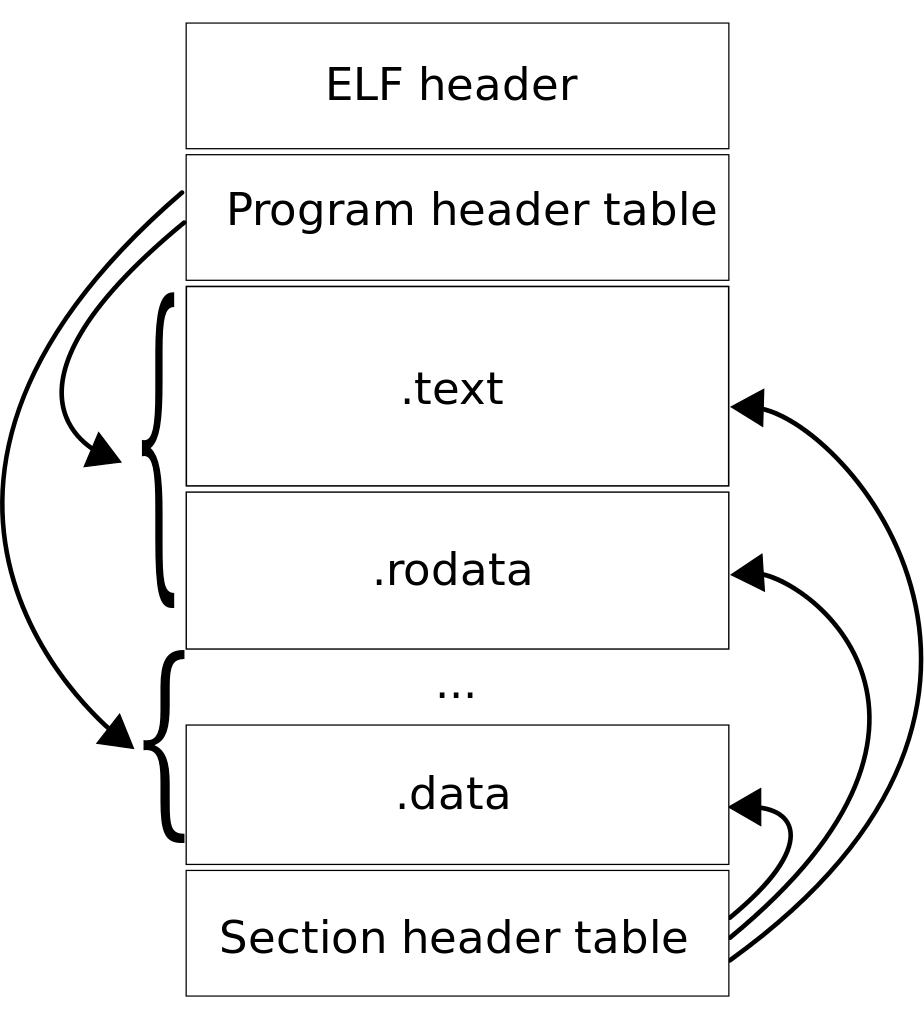
\includegraphics[scale=0.2]{./ELF.png}
				\label{fig:ELF}
				\caption{ELF Structures and Internal Linking}
			\end{figure}
			\begin{description}
				\item[Program Header Table:] This is a description and mapping of memory segments used in the program. 
					These could either be different modules of the program, or simply a divider for code and data. 
				\item[Section Header Table:] Describes the programs sections (such as .code or .data).
				\item[The Data Referred to by these Tables:] This is either the code or data itself which is described 
					and pointed to by thee above tables. 
			\end{description}

			These files are then linked to libraries, which are installed on the system to provide a given function to multiple programs\footnote{\url{http://tldp.org/HOWTO/Program-Library-HOWTO/shared-libraries.html}}.
			These libraries mean that program ELF files can be small, as they do not have to contain the code required to conduct all tasks. 
			However, it also means that there is another attack point and a dependency on the system.

			Libraries are usually found in ``/usr/lib/'', and named libxxx.so. 
			These files contain the code for core functions which are often used by a number of programs. 
			When programming, once the expected header file has been included, using a library is as simple as calling a method as if you had written it in your code. 

			For these cases, when the program is compiled, a separate program known as a ``linker'' will create the required pointers within the ELF output, allowing the program to call libraries on any system it is placed on. 
			This system means that the header sections of ELF files often refer to files and functions which do not exist within the ELF itself\footnote{\url{http://www.yolinux.com/TUTORIALS/LibraryArchives-StaticAndDynamic.html}}. 

			There are a number of tools which have been written to help working with ELF files:
			\begin{description}
				\item[readelf] Information gathering for ELF files. 
					Similar, but more detailed than objdump. 
				\item[objdump] Provides information and disassembly for object (and ELF) files. 
				\item[file] Attempt to determine type and information about a given file. 
					This will give some data on how the program was compiled. 
			\end{description}

		\subsection{Mach-O}
			Mach Object (or Mach-O) is the executable file format used on OS X, NeXTSTEP (which OS X was based on) and iOS. 
			As with ELF files, these are used for object code, shared libraries, linked code and core dumps\footnote{\url{https://developer.apple.com/library/mac/documentation/DeveloperTools/Conceptual/MachORuntime/index.html}}.

			The file is made up of the header, followed by load commands which provide the system with the files and data that must be loaded for the system to be able to execute the code found within. 
			This is followed by a number of sections, similar to those of ELF files. 

			These files can also be formed into one binary that is able to be executed on multiple architectures. 
			This is useful on systems such as iOS, which must have 4 different versions of the ARM architecture to run on all devices. 

			As with ELF above, these files are dynamically linked, requiring the relevant ``.dylib'' files to exist on the system. 
			
			While the same tools as with Linux will work, otool specific to Mach-O files\footnote{\url{https://www.objc.io/issues/6-build-tools/mach-o-executables/}}.
			It is an object file displaying tool that works in a similar way to objdump, but can be told to just give header information. 

		\subsection{Windows Portable Executable}
			\begin{wrapfigure}{I}{0.45\textwidth}
				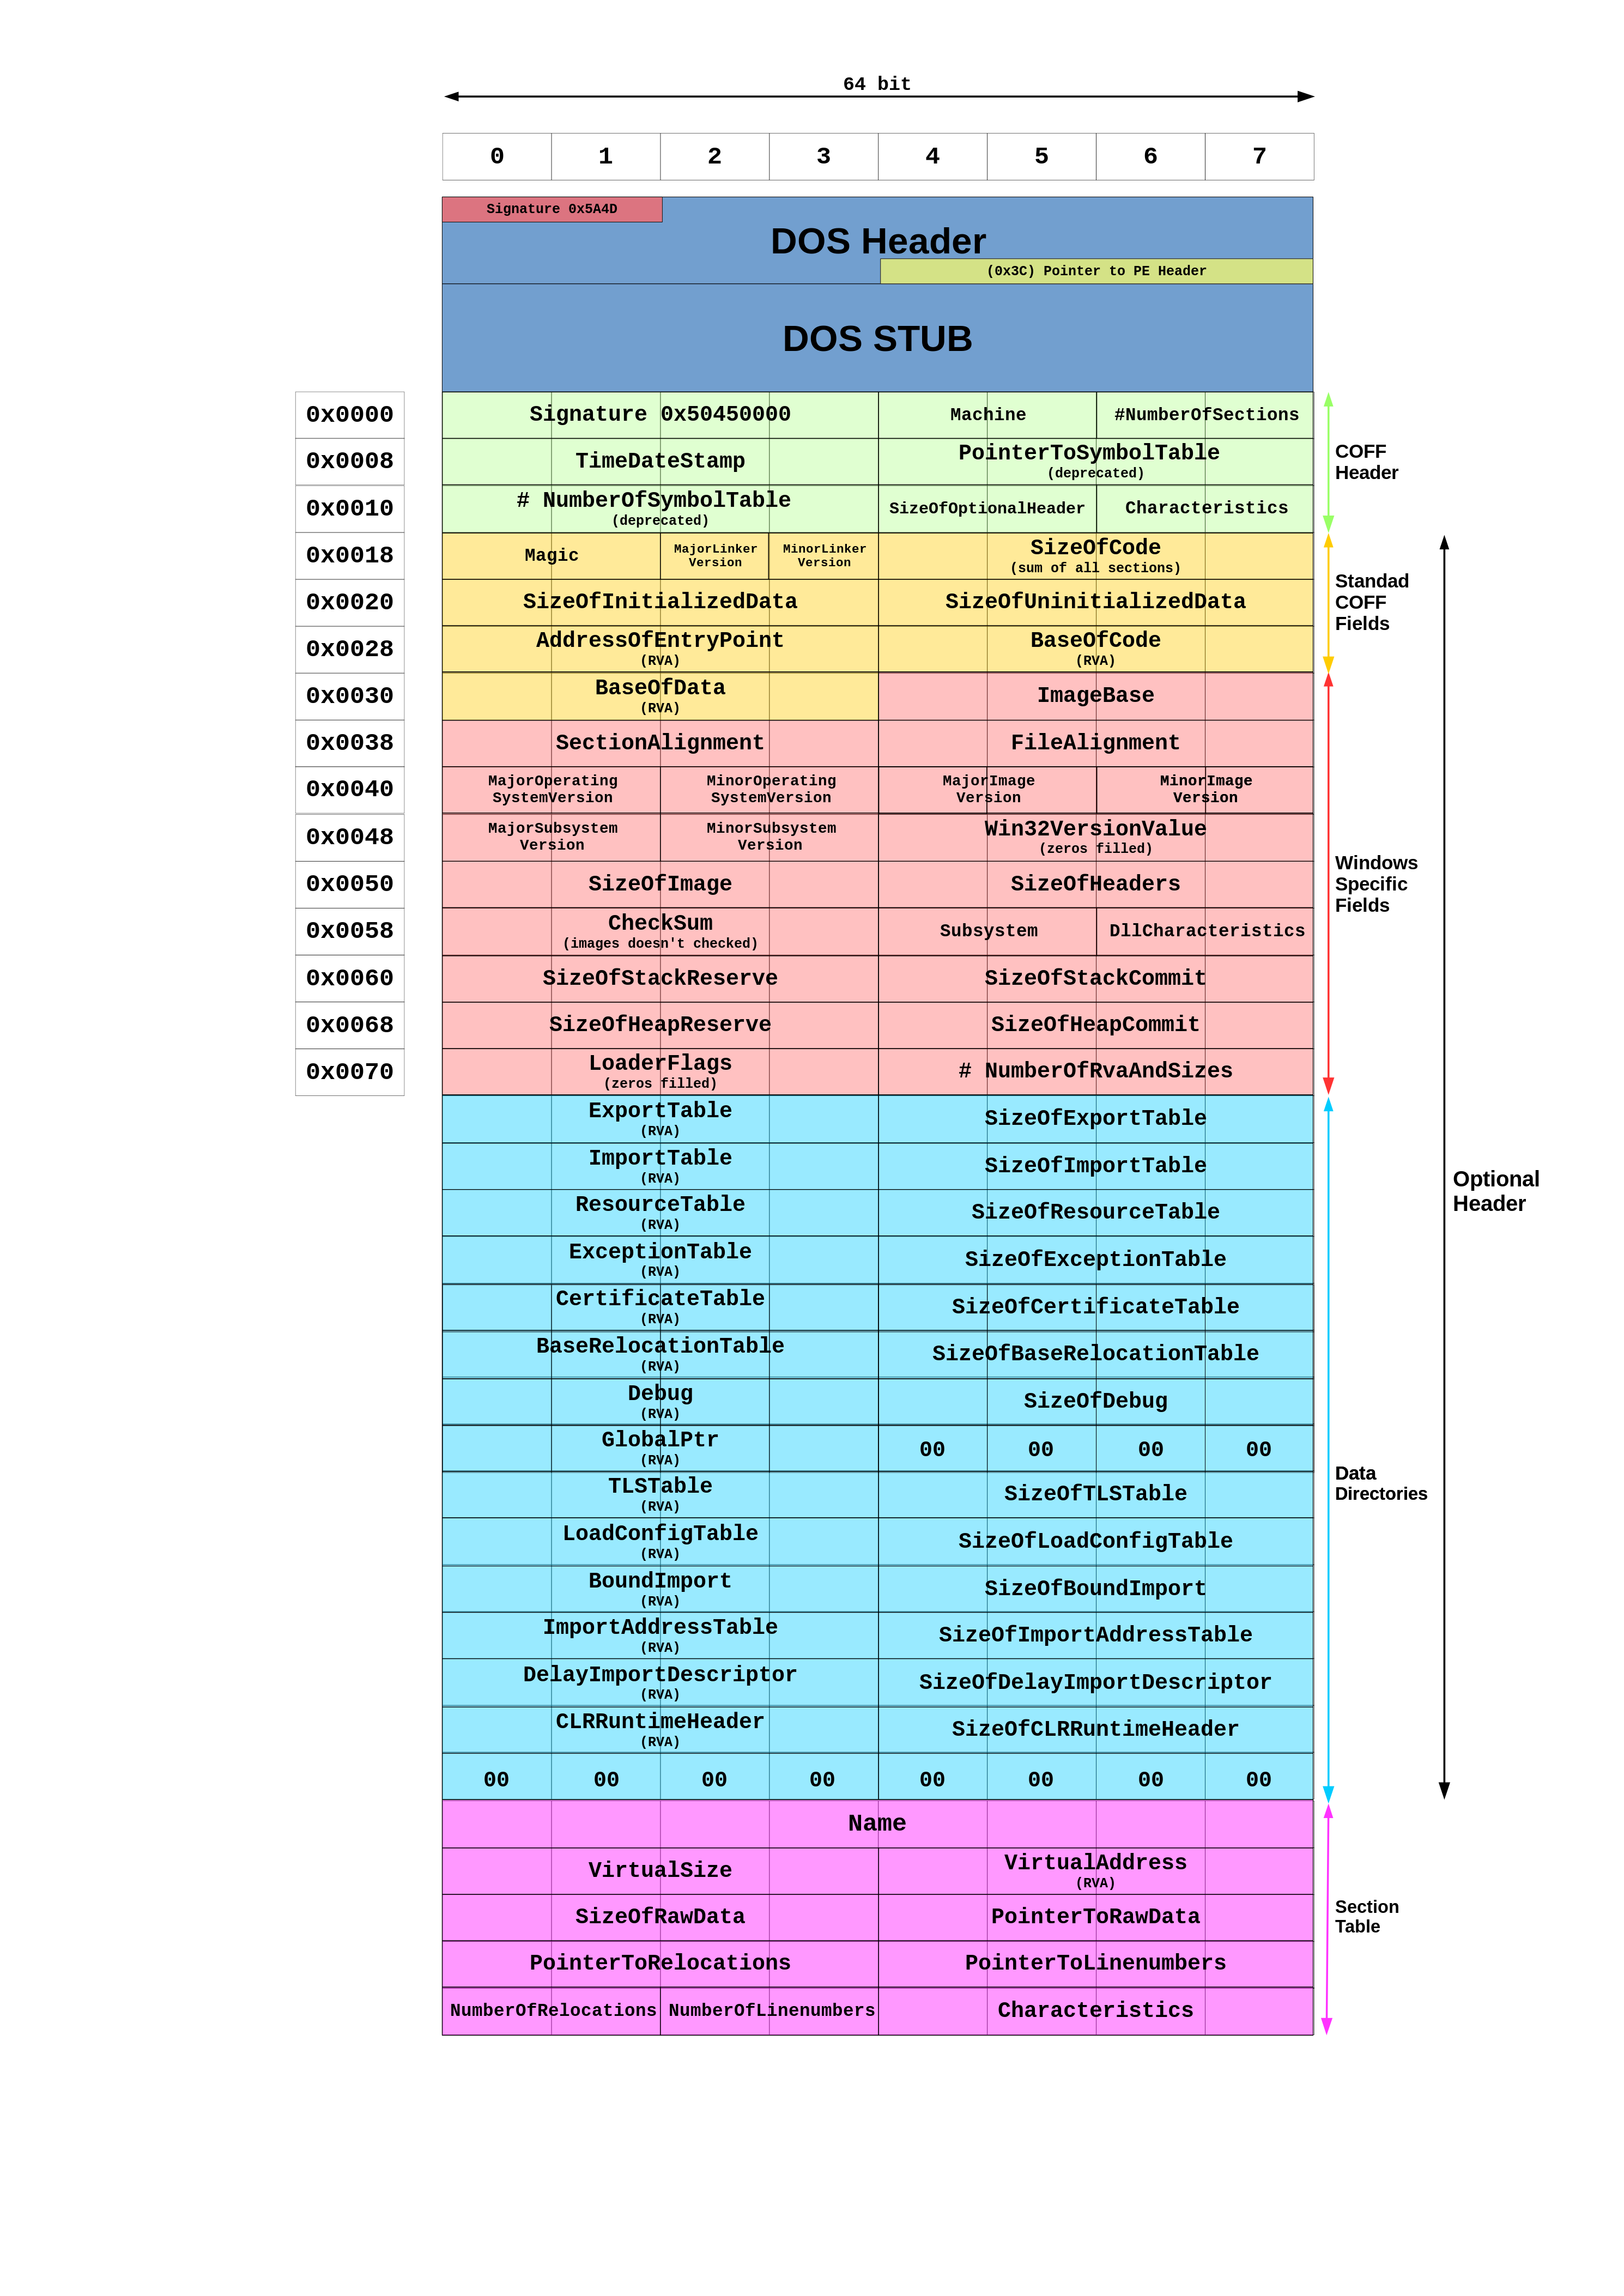
\includegraphics[width=0.43\textwidth]{./PE.png}
				\label{fig:PortableExecutable}
				\caption{Layout of Windows Portable Executable Files}
			\end{wrapfigure}
			Portable Executable (PE) is the Windows executable format. 
			It is based on the older UNIX COFF format, which was eventually replaced with ELF. 
			These files are commonly found within ``.exe'' and ``.DLL'' files on windows, as these are the executable 
			package and dynamically linked libraries on this system. 

			This format retains some legacy DOS support in that a DOS header is placed at the top of the file. 
			This header can either contain a full DOS version of the program, or simply a stub informing the user that the program is not DOS compatible. 

			The format for these files can be seen in figure \ref{fig:PortableExecutable}. 
			The headers within this file describe to the linker how to map the file and it's required libraries into memory. 
			It also specifies execute and read permissions for that memory, for example, code is usually executable and read only, while data is usually non-executable but read/write. 
			
			A lookup table is also implemented in the import table. 
			This table allows the PE file to call on shared libraries found on the system. 
			It is also a good point of attack as we can change the files or locations pointed to by this table. 

			It is also worth noting that the PE format does not implement position independent code. 
			This means that addresses within the file must be recalculated each time the code is loaded,
			in contrast with ELF files, which usually implement fully position independent code. 
			
